\documentclass[12pt]{article}

\raggedbottom

\usepackage{sbc-template}
\usepackage{graphicx,url}
\usepackage[utf8]{inputenc}
\usepackage[brazil]{babel}
\usepackage{amsmath}
\usepackage{listings}
\usepackage{xcolor}
\usepackage{float}

\lstset{
    language=C++,
    basicstyle=\ttfamily\footnotesize,
    keywordstyle=\color{blue},
    stringstyle=\color{red},
    commentstyle=\color{gray},
    numbers=left,
    numberstyle=\tiny,
    stepnumber=1,
    breaklines=true,
    frame=single,
    captionpos=b
}

\sloppy

\title{A Digital Clockwork Simulator: Simulação de Circuitos Digitais Discretos em C++ com Suporte Multiplataforma}

\author{
  Francisco Passos dos S. Alves\inst{1},
  João Vitor V. Leão\inst{1},
  Karlos Danyel S. Gomes\inst{1}, \\
  Lucca Pedreira Dultra\inst{1}
}

\address{
  Departamento de Computação -- Universidade Federal de Sergipe (UFS)\\
  São Cristóvão -- SE -- Brasil\\
  \email{\{francisco.alves, joao.leao2, karlos.gomes2, lucca.dultra\}@dcomp.ufs.br}
}

\begin{document}

\maketitle

\begin{abstract}
This paper describes the development of \textit{A Digital Clockwork Simulator}, a software simulator of a digital clock and alarm circuit, inspired by a discrete-logic hardware project by Wagner Rambo (WR Kits channel). The simulator was implemented in C++ following the object-oriented programming paradigm, with each integrated circuit modeled as an independent class that faithfully replicates the pin-level behavior described in the respective datasheet — including clock-edge dependencies, carry propagation, and asynchronous resets. The CD4000-series CMOS chips covered are: CD4029, CD4511, CD4017, CD4040, CD4013, CD4063, CD4081, and CD4071. As a course extension, a complete alarm subsystem (\textit{The Amazing Digital Alarm}) was developed, integrating cascaded magnitude comparators and D flip-flops for programmed-time storage and real-time comparison. The project also adopts a cross-platform architecture for keyboard input and audio output, with one implementation file per operating system (Linux, Windows, and macOS) compiled selectively by the Makefile behind platform-agnostic interfaces. The simulator is distributed under the GNU General Public License (GPL) and is publicly available on GitHub.
\end{abstract}

\begin{resumo}
Este artigo descreve o desenvolvimento de \textit{A Digital Clockwork Simulator}, um simulador de software de um circuito de relógio digital e alarme, inspirado em um projeto de hardware com lógica discreta de Wagner Rambo (canal WR Kits). O simulador foi implementado em C++ seguindo o paradigma de Programação Orientada a Objetos, com cada circuito integrado modelado como uma classe independente que replica fielmente o comportamento em nível de pino descrito no respectivo \textit{datasheet} — incluindo dependências de borda de \textit{clock}, propagação de \textit{carry} e resets assíncronos. Os chips CMOS da série CD4000 abrangidos são: CD4029, CD4511, CD4017, CD4040, CD4013, CD4063, CD4081 e CD4071. Como extensão da disciplina, foi desenvolvido um subsistema de alarme completo (\textit{The Amazing Digital Alarm}), integrando comparadores de magnitude cascateados e flip-flops D para armazenamento de horário programado e comparação em tempo real. O projeto adota ainda uma arquitetura multiplataforma para captura de teclado e saída de áudio, com um arquivo de implementação por sistema operacional (Linux, Windows e macOS) compilado seletivamente pelo Makefile, por trás de interfaces agnósticas de plataforma. O simulador é distribuído sob a licença GNU General Public License (GPL) e está disponível publicamente no GitHub.
\end{resumo}

% =============================================================
\section{Introdução}
% =============================================================

O estudo de sistemas digitais compreende a transição fundamental entre a abstração da álgebra booleana e a implementação física de circuitos eletrônicos~\cite{tocci}. Projetos que exigem a integração de componentes discretos — contadores, decodificadores, flip-flops e comparadores — são particularmente eficazes para consolidar essa transição, pois obrigam o estudante a raciocinar simultaneamente sobre sinais individuais, bordas de \textit{clock} e propagação de estados ao longo de uma cadeia de chips.

\textit{A Digital Clockwork Simulator} foi desenvolvido com esse objetivo: reproduzir, em software, o comportamento lógico de um relógio digital de lógica discreta projetado por Wagner Rambo e disponibilizado em seu canal no YouTube, WR Kits~\cite{rambo:15}. O simulador foi implementado em linguagem C++ utilizando o paradigma de Programação Orientada a Objetos (POO), modelando cada circuito integrado como uma classe independente cujos métodos correspondem diretamente às operações descritas nos \textit{datasheets} dos respectivos componentes.

A abordagem adotada caracteriza-se pela fidelidade ao nível de pino do hardware: não são introduzidas abstrações de software que não encontrem equivalente no circuito físico. Se o hardware exigiria dois pulsos de \textit{clock} sequenciais em chips distintos, a simulação aplica exatamente dois pulsos sequenciais. Essa escolha, além de pedagogicamente relevante, torna o código diretamente rastreável ao esquemático original, facilitando a compreensão da relação entre o comportamento lógico simulado e o comportamento elétrico real.

Como extensão do escopo original, requisitada pela disciplina de Sistemas Digitais, o projeto incorpora um subsistema de alarme completo — denominado \textit{The Amazing Digital Alarm} — que integra comparadores de magnitude cascateados, flip-flops D e lógica de validação de dia da semana. O conjunto foi ainda evoluído para suporte multiplataforma (Linux, Windows e macOS), mantendo o módulo de simulação inteiramente independente do sistema operacional hospedeiro.

O projeto é distribuído sob a licença GNU General Public License (GPL) e está disponível publicamente no GitHub\footnote{\url{https://github.com/FrankSteps/digital-clockwork-simulator}}.

% =============================================================
\section{Fundamentação Teórica e Componentes}
% =============================================================

A família CMOS CD4000 reúne circuitos integrados de baixo consumo, ampla faixa de tensão de alimentação e comportamento lógico bem definido em \textit{datasheets} públicos~\cite{floyd}. Essa padronização torna os componentes da série especialmente adequados para fins educacionais: cada pino possui função inequívoca, e a cascata entre chips obedece a regras de temporização estáveis. No simulador, cada CI foi implementado como uma classe C++ em \texttt{include/chips.hpp} e \texttt{src/chips.cpp}, com os métodos públicos correspondendo diretamente aos pinos e operações do \textit{datasheet}.

O \textbf{CD4029}~\cite{ti:cd4029} é um contador BCD \textit{Up/Down} presettable de 4 bits, empregado na contagem das unidades e dezenas de minutos e horas. O mecanismo de \textit{ripple carry} foi modelado para que cada contador subsequente receba o pulso de \textit{Carry In} apenas quando o anterior gerar \textit{Carry Out} — replicando fielmente a cascata que ocorreria entre chips físicos e que, segundo~\cite{tocci}, é a base da contagem multidígito em sistemas BCD.

O \textbf{CD4511}~\cite{ti:cd4511} é o decodificador BCD para display de sete segmentos responsável por converter as saídas binárias dos CD4029 nos sinais que ativam cada segmento do display renderizado no terminal. A implementação reproduz os três pinos de controle definidos no \textit{datasheet}: \textit{Lamp Test} (LE), \textit{Blanking} (BL) e \textit{Latch Enable} (LE), permitindo que o display possa ser habilitado, apagado ou congelado independentemente da contagem em andamento.

O \textbf{CD4017}~\cite{ti:cd4017} é um contador Johnson de dez estágios que, no projeto, é instanciado de duas formas distintas: no módulo de relógio, configurado com limite de reset em 2 para funcionar como indicador de meridiano (AM/PM); e no módulo de alarme, configurado com limite de reset em 7 para implementar o contador de dias da semana. Essa reutilização do mesmo componente em funções diferentes ilustra a flexibilidade proporcionada pela configuração programática do limite de contagem.

O \textbf{CD4040}~\cite{ti:cd4040} é um divisor de frequência ripple de 12 estágios. No simulador, recebe o sinal de 60\,Hz produzido pelo \texttt{FreqGenerator} e fornece, em suas saídas $Q_n$, subfrequências binárias decrescentes que são utilizadas nos modos de ajuste lento e rápido do relógio. A combinação de duas saídas do CD4040 por portas AND do CD4081 produz o pulso que avança os contadores no modo padrão de operação.

O \textbf{CD4013}~\cite{ti:cd4013} é um flip-flop D duplo de borda positiva. Conforme descrito em~\cite{floyd}, flip-flops D são os elementos básicos de armazenamento em sistemas digitais síncronos: a saída $Q$ assume o valor da entrada $D$ somente na borda ativa do \textit{clock}, permanecendo estável entre bordas. No módulo de alarme, 9 instâncias do CD4013 (18 flip-flops individuais) armazenam o horário programado: 16 bits de tempo em BCD (HH:MM), 1 bit de meridiano e 1 bit de estado de armamento (\textit{stand-by}).

O \textbf{CD4063}~\cite{ti:cd4063} é um comparador de magnitude de 4 bits com entradas de cascata (\textit{Equal}, \textit{Greater}, \textit{Smaller}). Cinco instâncias são cascateadas no módulo de alarme para comparar o horário armazenado nos flip-flops com o barramento de tempo atual, propagando os sinais de comparação da unidade de minutos até o meridiano — exatamente como seria feito em hardware físico para comparações de palavras maiores que 4 bits~\cite{tocci}.

O \textbf{CD4081}~\cite{ti:cd4081} (quatro portas AND de 2 entradas) e o \textbf{CD4071}~\cite{ti:cd4071} (quatro portas OR de 2 entradas) são empregados em duas funções distintas: na lógica de reset assíncrono dos contadores de horas, detectando condições de overflow específicas; e na redução lógica do comparador de dias da semana, em que sete sinais AND individuais (um por dia) são combinados por uma cascata de portas OR até produzir um único sinal de validação.

\subsection{Gerador de Frequência}

No projeto original de Wagner Rambo~\cite{rambo:15}, o \textit{clock} do relógio é derivado diretamente da rede elétrica brasileira (60\,Hz): um transformador reduz a tensão da rede para o nível lógico de operação, e um circuito de condicionamento de sinal converte a senoide resultante em um sinal digital de onda quadrada, aproveitando simultaneamente a frequência e a tensão da rede sem necessidade de um oscilador dedicado~\cite{mamede}.

No simulador, esse papel é desempenhado pela classe \texttt{FreqGenerator} (\texttt{include/freqGenerator.hpp}, \texttt{src/freqGenerator.cpp}). Uma \textit{thread} dedicada alterna o sinal lógico a cada meio período de 60\,Hz, utilizando \texttt{std::this\_thread::sleep\_until} ancorado em pontos de tempo absolutos — estratégia que compensa atrasos acumulados ao longo da execução e reduz a deriva temporal em relação a abordagens baseadas em \texttt{sleep\_for}. O sinal é entregue diretamente como onda quadrada, uma vez que sinais senoidais não possuem representação em lógica digital discreta: a conversão que o circuito de condicionamento realizaria no hardware é assumida como pré-existente na abstração do simulador.

% =============================================================
\section{Arquitetura e Implementação}
% =============================================================

O simulador é organizado em dois grandes módulos de simulação interligados: o \textit{A Digital Clockwork}, responsável pela geração e manutenção do tempo, e o \textit{The Amazing Digital Alarm}, responsável pelo armazenamento do horário programado, pela comparação com o tempo atual e pelo disparo do alarme. A Figura~\ref{fig:simulator} apresenta a interface do simulador em execução no terminal (Linux).

\begin{figure}[htbp]
    \centering
    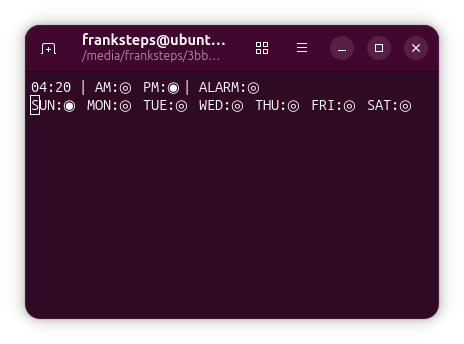
\includegraphics[width=0.72\textwidth]{./assets/a_digital_clockwork/simulator.png}
    \caption{Interface do \textit{A Digital Clockwork Simulator} renderizada no terminal (Linux).}
    \label{fig:simulator}

    \centering
    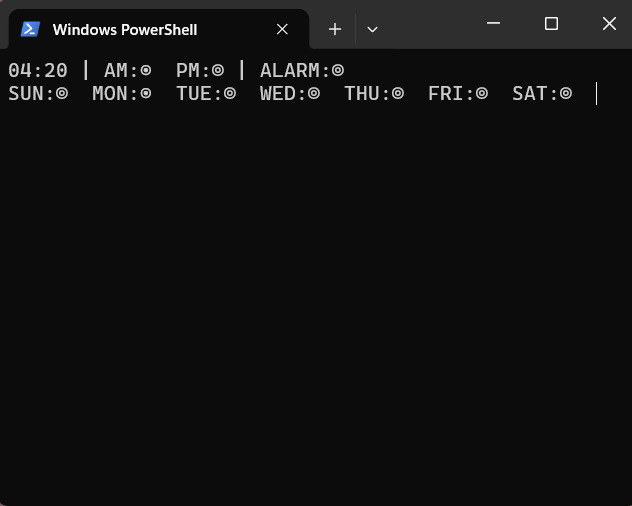
\includegraphics[width=0.72\textwidth]{./assets/a_digital_clockwork/win.jpeg}
    \caption{Interface no terminal (Windows).}
    \label{fig:win}
\end{figure}

\subsection{O Relógio — \textit{A Digital Clockwork}}

O módulo de relógio é implementado na classe \texttt{DigitalClockwork} (\texttt{include/digitalClockwork.hpp}, \texttt{src/digitalClockwork.cpp}). O \texttt{FreqGenerator} fornece o sinal de referência de 60 Hz, que é aplicado ao CD4040. Esse circuito integrado atua como um divisor de frequência ripple, produzindo em suas saídas sinais cujas frequências correspondem à frequência de entrada dividida por potências de dois. Essas saídas são combinadas pelas portas AND do CD4081 para gerar os pulsos responsáveis por avançar os contadores CD4029 nos diferentes modos de operação.

A contagem de tempo é realizada por quatro instâncias do CD4029, dispostas em cascata: unidade de minutos, dezena de minutos, unidade de horas e dezena de horas. O mecanismo de \textit{ripple carry} entre contadores é modelado no método \texttt{cascadeCount()}: o CD4029[0] (unidade de minutos) recebe o pulso de \textit{clock} diretamente; os demais só avançam se o anterior gerou \textit{Carry Out}, replicando o comportamento de cascata descrito em~\cite{tocci} para contadores multidígito.

Os resets assíncronos — necessários para reiniciar a dezena de minutos ao atingir 6 e para reiniciar as horas ao atingir 13 e retornar a 1 — são detectados pelo método \texttt{updateAND()}, que lê combinações específicas dos bits de saída dos CD4029 e aciona as portas AND do CD4081[0]. Quando a condição é satisfeita, \texttt{applyResets()} aplica o pulso de \textit{Preset Enable} ao contador correspondente — replicando o comportamento de reset assíncrono por realimentação de saídas, amplamente documentado em projetos de relógio digital com lógica discreta~\cite{floyd}. A Figura~\ref{fig:counter} ilustra o diagrama esquemático dessa lógica.

\begin{figure}[H]
    \centering
    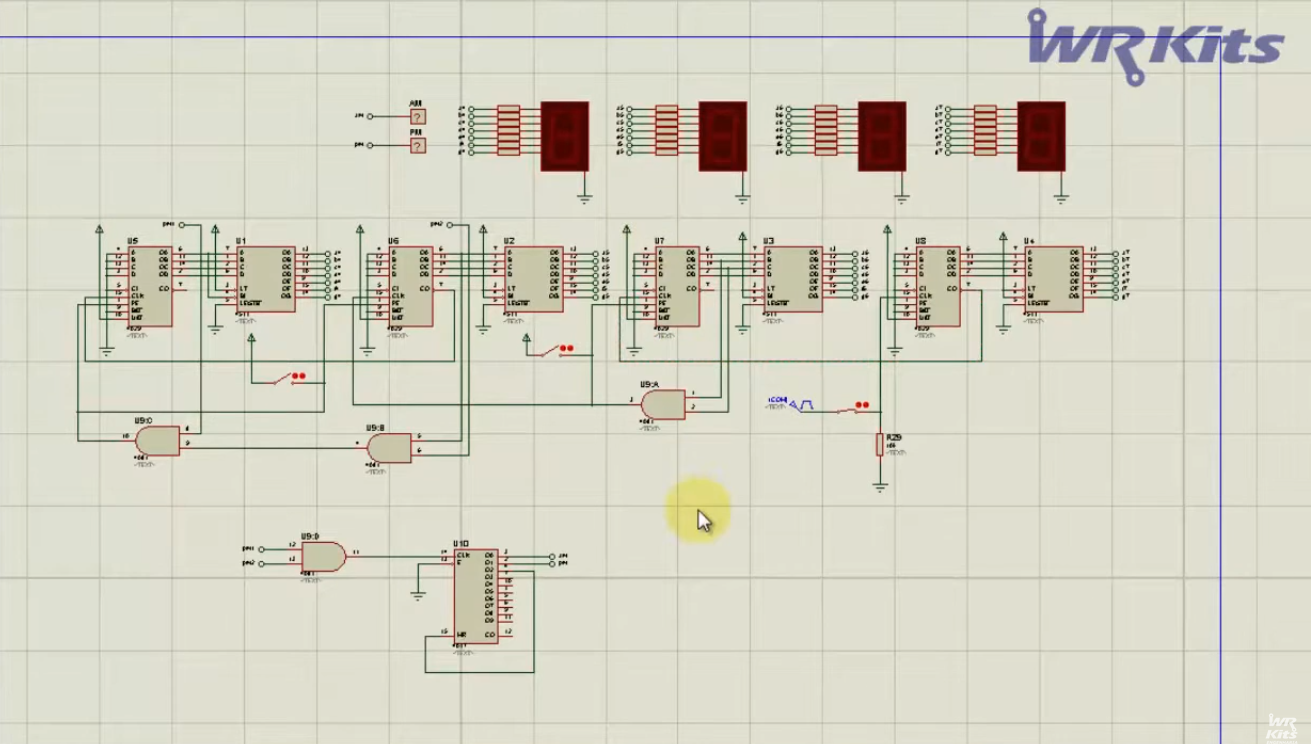
\includegraphics[width=0.78\textwidth]{./assets/a_digital_clockwork/counter.png}
    \caption{Diagrama esquemático do módulo de contagem do relógio digital.}
    \label{fig:counter}
\end{figure}

A seleção da frequência de avanço do contador segundo o modo de operação (padrão, lento ou rápido) é realizada pelo método \texttt{frequencyConverter()}, apresentado na Listagem~\ref{lst:frequencyConverter}. No modo padrão (\texttt{DEFAULT}), a saída combinada das portas AND do CD4081[1] produz um pulso por minuto; nos modos de ajuste, as saídas $Q_0$ e $Q_5$ do CD4040 fornecem, respectivamente, frequências mais elevadas para ajuste rápido e mais reduzidas para ajuste lento. A detecção de borda — condição \texttt{Q \&\& !lastQ} — garante que o contador avance apenas uma vez por transição positiva, evitando múltiplos incrementos por nível lógico alto.

\begin{lstlisting}[caption={Seleção de frequência por modo de ajuste em \texttt{DigitalClockwork}.}, label={lst:frequencyConverter}]
void DigitalClockwork::frequencyConverter(ADJUSTMENT MODE){
    bool Q0 = cd4040.getOutput(0);
    bool Q5 = cd4040.getOutput(5);

    updateAND_1();
    bool Out4081 = cd4081[1].getOutput(2);

    switch(MODE){
        case ADJUSTMENT::FAST:
            if(Q0 && !lastQ0){
                updateCounter();
            }
            break;
        case ADJUSTMENT::SLOW:
            if(Q5 && !lastQ5){
                updateCounter();
            }
            break;
        case ADJUSTMENT::DEFAULT:
            if(Out4081 && !lastOut4081 && defaultCooldown == 0){
                updateCounter();
                defaultCooldown = 500;
            }
            if(defaultCooldown > 0) defaultCooldown--;
            break;
    }
    lastQ0 = Q0;
    lastQ5 = Q5;
    lastOut4081 = Out4081;
}
\end{lstlisting}

\subsection{O Alarme — \textit{The Amazing Digital Alarm}}

O módulo de alarme é implementado na classe \texttt{DigitalAlarm} (\texttt{include/digitalAlarm.hpp}, \texttt{src/digitalAlarm.cpp}), integrando lógica combinacional e sequencial em torno de três caminhos independentes: memória de horário, comparação de tempo e comparação de dia da semana. O esquema lógico estrutural completo é apresentado na Figura~\ref{fig:alarm}.

\begin{figure}[H]
    \centering
    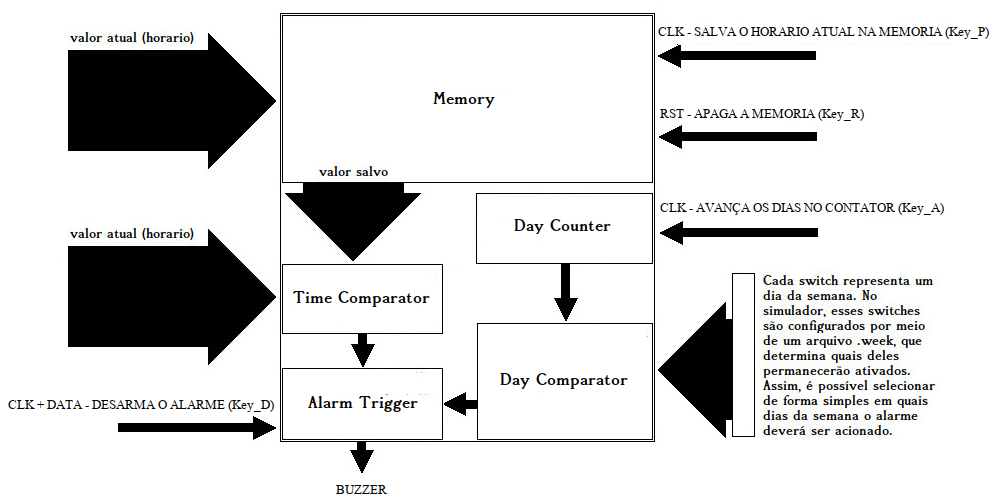
\includegraphics[width=0.90\textwidth]{./assets/the_amazing_digital_alarm/project.png}
    \caption{Esquema lógico estrutural do \textit{Amazing Digital Alarm}.}
    \label{fig:alarm}
    \vspace{0.1cm} 
    {\small \textbf{Fonte:} Autoria própria.}
\end{figure}

\subsubsection{Memória de Horário}

O armazenamento do horário programado utiliza 9 instâncias do CD4013~\cite{ti:cd4013} — 18 flip-flops D individuais — distribuídas da seguinte forma: 16 bits para o tempo HH:MM em BCD (bits 0 a 15), 1 bit de meridiano (bit 16) e 1 bit de estado de armamento (\textit{stand-by}), no flip-flop 1 do CD4013[8]. A separação entre a atualização das entradas D e a captura efetiva pela borda de \textit{clock} é um aspecto central da implementação: o método \texttt{setDataMemory()} atualiza continuamente as entradas D de todos os flip-flops a cada ciclo, sem aplicar pulsos, mantendo o barramento de tempo atual ``à porta'' da memória; apenas quando o método \texttt{programAlarm()} é invocado (tecla P) os pulsos de \textit{clock} são aplicados simultaneamente a todos os flip-flops, capturando o horário exibido naquele instante. Esse comportamento replica diretamente o mecanismo de \textit{latch} descrito em~\cite{floyd} para flip-flops D em modo de captura síncrona. A Figura~\ref{fig:memory} ilustra o caminho de dados da memória.

\begin{figure}[H]
    \centering
    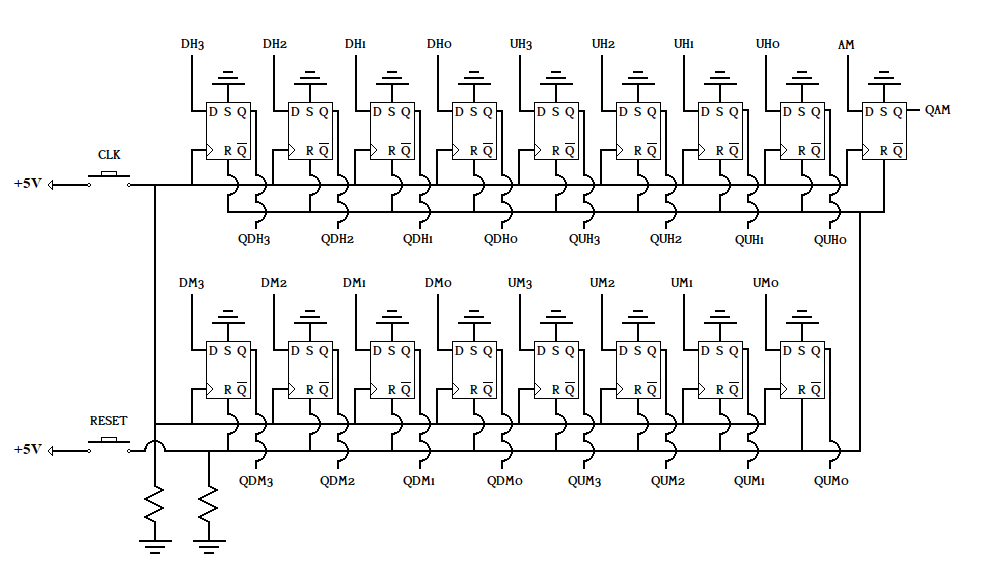
\includegraphics[width=0.78\textwidth]{./assets/the_amazing_digital_alarm/memory.png}
    \caption{Diagrama do módulo de memória do alarme (CD4013).}
    \label{fig:memory}
    \vspace{0.1cm} 
    {\small \textbf{Fonte:} Autoria própria.}
\end{figure}

\subsubsection{Comparação de Tempo}

A comparação entre o horário armazenado nos flip-flops e o barramento de tempo atual é realizada por uma cascata de cinco instâncias do CD4063~\cite{ti:cd4063}. O CD4063[0] compara a unidade de minutos; CD4063[1], a dezena de minutos; CD4063[2] e CD4063[3], a unidade e a dezena de horas; CD4063[4] compara o bit de meridiano. Em cada estágio, as saídas \textit{Equal}, \textit{Greater} e \textit{Smaller} do estágio anterior são conectadas às entradas de cascata do estágio seguinte — o mesmo procedimento descrito em~\cite{tocci} para extensão da comparação a palavras maiores que 4 bits. O sinal de igualdade final do CD4063[4] indica que o horário programado coincide com o tempo atual. A Figura~\ref{fig:time_comparator} detalha esse caminho.

\begin{figure}[H]
    \centering
    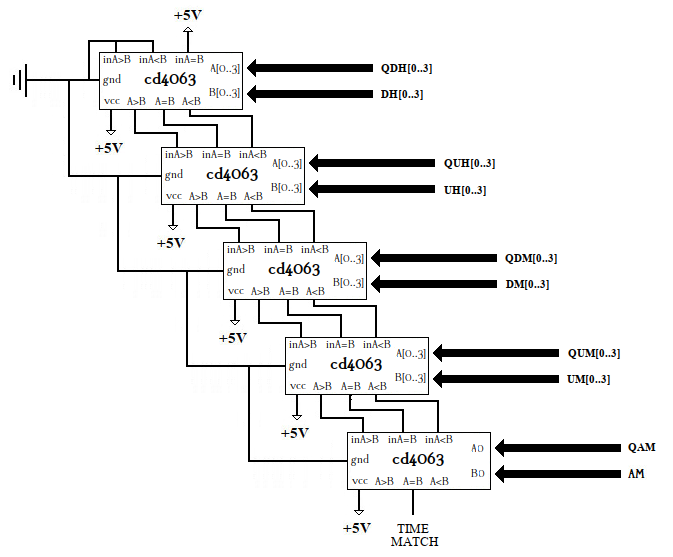
\includegraphics[width=0.78\textwidth]{./assets/the_amazing_digital_alarm/time_comparator.png}
    \caption{Cascata de comparadores de magnitude CD4063 para validação de horário.}
    \label{fig:time_comparator}
    \vspace{0.1cm} 
    {\small \textbf{Fonte:} Autoria própria.}
\end{figure}

\subsubsection{Comparação de Dia da Semana}

A configuração dos dias em que o alarme deve ser ativado é realizada por meio de um arquivo \texttt{.week}, que simula sete chaves DIP físicas ON/OFF — uma por dia da semana. O método \texttt{loadWeekFile()} realiza a leitura e validação rigorosa do arquivo: são rejeitados arquivos com extensão incorreta, linhas malformadas, valores fora do domínio $\{0,1\}$ e dias declarados fora da ordem esperada (SUN a SAT). A validação de dia no alarme combina a saída ativa do CD4017 (indicando o dia corrente) com o valor da chave correspondente do arquivo \texttt{.week} por meio de portas AND do CD4081; em seguida, uma cascata de portas OR do CD4071 reduz os sete sinais AND a um único sinal de ``dia habilitado''. A Figura~\ref{fig:day_comparator} ilustra essa lógica.

\begin{figure}[H]
    \centering
    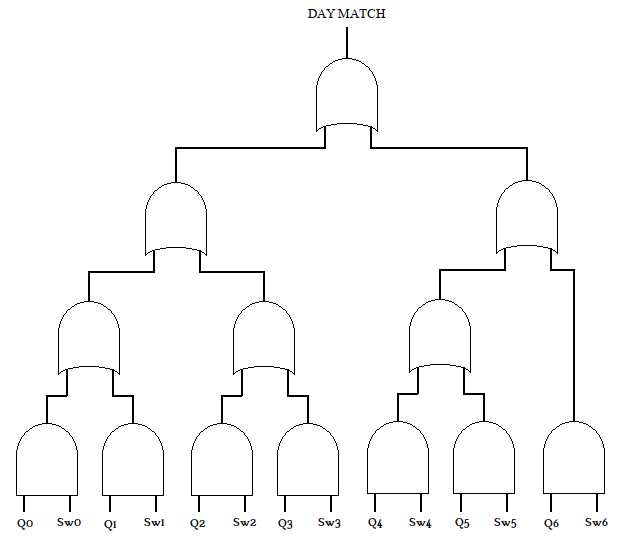
\includegraphics[width=0.78\textwidth]{./assets/the_amazing_digital_alarm/day_comparator.png}
    \caption{Lógica de comparação de dia da semana com CD4081 e CD4071.}
    \label{fig:day_comparator}
    \vspace{0.1cm} 
    {\small \textbf{Fonte:} Autoria própria.}
\end{figure}

\subsubsection{Disparo e Desarmamento}

A saída final do alarme resulta da combinação, por uma porta AND do CD4081[2], de três sinais independentes: o sinal de ``dia habilitado'', o sinal de igualdade de tempo e o sinal de \textit{stand-by} (flip-flop 1 do CD4013[8]). O resultado é então combinado com o sinal $Q_6$ do CD4040, proveniente do \textit{Digital Clockwork}, produzindo um pulso rítmico que aciona o \texttt{Buzzer} de forma intermitente. O desarmamento é realizado pela tecla D (\textit{Disarm}), que aplica reset no flip-flop de \textit{stand-by}, interrompendo a saída; a tecla R (\textit{Reset}) apaga integralmente a memória, aplicando reset em todos os 18 flip-flops. A Figura~\ref{fig:alarm_trigger} ilustra o circuito de disparo e desarmamento.

\begin{figure}[H]
    \centering
    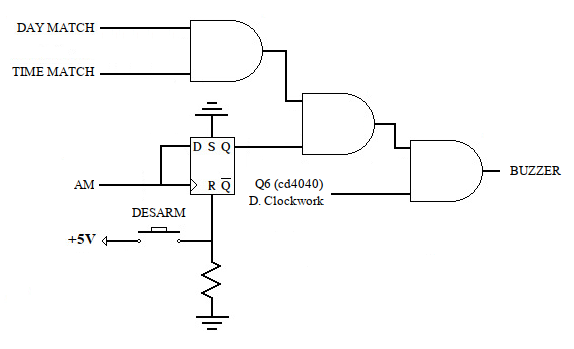
\includegraphics[width=0.78\textwidth]{./assets/the_amazing_digital_alarm/alarm_trigger.png}
    \caption{Circuito de disparo e desarmamento do alarme.}
    \label{fig:alarm_trigger}
    \vspace{0.1cm} 
    {\small \textbf{Fonte:} Autoria própria.}
\end{figure}

\subsection{Interface de Terminal e Entrada de Teclado}

Todo o estado lógico simulado é refletido em tempo real no terminal do sistema operacional pelas classes \texttt{Display} e \texttt{Led} (\texttt{include/feedback.hpp}, \texttt{src/feedback.cpp}). O \texttt{Display} converte as saídas dos CD4511 em dígitos de sete segmentos renderizados em caracteres ASCII; os indicadores \texttt{Led} exibem o meridiano (AM/PM), o dia ativo no CD4017 e o estado de armamento do alarme por meio dos símbolos \texttt{\textbullet} (ligado) e \texttt{\textopenbullet} (desligado).

A captura de teclado segue o mesmo princípio arquitetural aplicado aos demais módulos dependentes de plataforma: uma interface comum declarada em \texttt{include/keyboard.hpp} expõe as funções \texttt{initKeyboard()}, \texttt{pollKeys()} e \texttt{closeKeyboard()}, implementadas separadamente em \texttt{src/keyboard\_linux.cpp} (via \texttt{libevdev}, lendo eventos brutos do kernel em \texttt{/dev/input/eventX}), \texttt{src/keyboard\_windows.cpp} (via \texttt{GetAsyncKeyState} da WinAPI, com \textit{polling} global independente de foco de janela) e \texttt{src/keyboard\_macintosh.cpp} (via \texttt{CGEventTap} de \textit{ApplicationServices}, \textit{event tap} em nível de sistema). O \texttt{main.cpp} invoca exclusivamente as funções da interface e permanece idêntico nas três plataformas.

\subsection{Saída de Áudio}

O \texttt{Buzzer}, declarado em \texttt{include/audio\_output.hpp}, segue a mesma arquitetura de interface comum com implementação por plataforma. No Linux, \texttt{src/audio\_output\_linux.cpp} utiliza ALSA (\texttt{libasound}) com escritas bloqueantes via \texttt{snd\_pcm\_writei}; no Windows, \texttt{src/audio\_output\_windows.cpp} utiliza WinMM (\texttt{waveOut*}) com buffers do tipo \texttt{WAVEHDR}; no macOS, \texttt{src/audio\_output\_macintosh.cpp} utiliza CoreAudio \texttt{AudioQueue}, cujo modelo orientado a \textit{callback} difere estruturalmente das abordagens bloqueantes das outras plataformas, embora a interface pública do \texttt{Buzzer} permaneça idêntica.

O sinal sonoro gerado é uma onda quadrada de 2000\,Hz pré-calculada no construtor: o \texttt{soundBuffer} alterna entre os valores $+32767$ e $-32767$ (máximo e mínimo de um \textit{short} de 16 bits com sinal) a cada meio período, produzindo o bipe característico de um buzzer eletrônico. Uma \textit{thread} dedicada alterna continuamente entre a escrita do \texttt{soundBuffer} e do \texttt{silenceBuffer} (todo zeros) conforme o estado do sinal lógico recebido via \texttt{setState()}. O controle de concorrência entre a \textit{thread} do buzzer e o restante do programa é realizado com \texttt{std::atomic<bool>} — escolha intencional em relação ao \texttt{mutex}, pois as variáveis de controle (\texttt{running} e \texttt{state}) são lidas e escritas de forma isolada, sem necessidade de atomicidade entre operações múltiplas, tornando a instrução atômica de CPU a solução correta e mais eficiente para esse caso.

\subsection{Seleção de Plataforma no Makefile}

A seleção dos arquivos de implementação específicos de cada plataforma é realizada em tempo de compilação pelo \textit{Makefile}, que detecta o sistema operacional via \texttt{uname -s} em Linux e macOS e via a variável de ambiente \texttt{\$(OS)} em Windows. Com base nessa detecção, as variáveis \texttt{KEYBOARD\_SRC}, \texttt{AUDIO\_SRC} e \texttt{CONSOLE\_SRC} recebem os arquivos corretos, e as \textit{flags} de linkagem são ajustadas de forma correspondente: \texttt{-lasound} e \texttt{-levdev} no Linux; \texttt{-framework AudioToolbox}, \texttt{-framework Carbon} e \texttt{-framework ApplicationServices} no macOS; e \texttt{-lwinmm} no Windows. O \texttt{main.cpp} permanece intocado e idêntico nas três plataformas — a portabilidade é resolvida inteiramente na camada de build, sem condicionais de pré-processador no código principal.

% =============================================================
\section{Conclusão}
% =============================================================

O desenvolvimento do \textit{A Digital Clockwork Simulator} demonstrou que a simulação orientada a objetos de circuitos digitais discretos constitui uma abordagem pedagogicamente eficaz para o estudo de sistemas digitais. A modelagem de cada CI como uma classe C++ independente, com métodos que refletem diretamente os pinos e operações definidos nos \textit{datasheets}~\cite{ti:cd4029,ti:cd4511,ti:cd4017,ti:cd4040,ti:cd4013,ti:cd4063,ti:cd4081,ti:cd4071}, exigiu compreensão aprofundada tanto do comportamento elétrico de cada componente quanto dos mecanismos de temporização e cascata que governam o funcionamento do circuito como um todo~\cite{tocci,floyd}.

A extensão com o \textit{Amazing Digital Alarm} forçou a integração de lógica combinacional e sequencial em escala significativa: 18 flip-flops D distribuídos em 9 instâncias do CD4013, 5 comparadores de magnitude CD4063 cascateados e uma rede de 4 chips CD4071 e CD4081 atuando em conjunto para produzir um único sinal de disparo bem definido. A implementação bem-sucedida desse subsistema evidencia que o domínio da abstração de arquiteturas digitais permite transpor diretamente a lógica de circuitos físicos para sistemas de software estruturados.

Por fim, a evolução do projeto para suporte multiplataforma — com implementações separadas por sistema operacional para teclado, áudio e configuração de terminal, todas compiladas seletivamente pelo \textit{Makefile} por trás de interfaces comuns — demonstrou que é possível manter um núcleo de simulação completamente agnóstico de plataforma sem recorrer a hierarquias de classes ou a condicionais de pré-processador no código principal. A portabilidade foi resolvida na camada de \textit{build}, preservando a legibilidade e a manutenibilidade do código de simulação.

% =============================================================
\begin{thebibliography}{99}

\bibitem[Tocci 2011]{tocci}
TOCCI, R. J.; WIDMER, N. S.; MOSS, G. L. \textit{Sistemas Digitais: Princípios e Aplicações}. 11.~ed. São Paulo: Pearson Prentice Hall, 2011.

\bibitem[Floyd 2007]{floyd}
FLOYD, T. L. \textit{Fundamentos de Sistemas Digitais}. 9.~ed. São Paulo: Pearson Prentice Hall, 2007.

\bibitem[Mamede 2012]{mamede}
MAMEDE FILHO, J. \textit{Manual de Equipamentos Elétricos}. 4.~ed. Rio de Janeiro: LTC, 2012.

\bibitem[Rambo 2015]{rambo:15}
RAMBO, W. \textit{Relógio Digital com Lógica Discreta CMOS}. Canal WR Kits (YouTube), 2015. Disponível em: \url{https://www.youtube.com/@WRKits}.

\bibitem[TI CD4029]{ti:cd4029}
TEXAS INSTRUMENTS. \textit{CD4029B Types: CMOS Presettable Up/Down Counter — Datasheet}. 2003. Disponível em: \url{https://www.ti.com/lit/ds/symlink/cd4029b.pdf}.

\bibitem[TI CD4511]{ti:cd4511}
TEXAS INSTRUMENTS. \textit{CD4511B Types: CMOS BCD-to-7-Segment Latch/Decoder/Driver — Datasheet}. 2003. Disponível em: \url{https://www.ti.com/lit/ds/symlink/cd4511b.pdf}.

\bibitem[TI CD4017]{ti:cd4017}
TEXAS INSTRUMENTS. \textit{CD4017B Types: CMOS Decade Counter/Divider — Datasheet}. 2003. Disponível em: \url{https://www.ti.com/lit/ds/symlink/cd4017b.pdf}.

\bibitem[TI CD4040]{ti:cd4040}
TEXAS INSTRUMENTS. \textit{CD4040B Types: CMOS 12-Stage Ripple-Carry Binary Counter/Divider — Datasheet}. 2003. Disponível em: \url{https://www.ti.com/lit/ds/symlink/cd4040b.pdf}.

\bibitem[TI CD4013]{ti:cd4013}
TEXAS INSTRUMENTS. \textit{CD4013B Types: CMOS Dual D-Type Flip-Flop — Datasheet}. 2003. Disponível em: \url{https://www.ti.com/lit/ds/symlink/cd4013b.pdf}.

\bibitem[TI CD4063]{ti:cd4063}
TEXAS INSTRUMENTS. \textit{CD4063B Types: CMOS 4-Bit Magnitude Comparator — Datasheet}. 2003. Disponível em: \url{https://www.ti.com/lit/ds/symlink/cd4063b.pdf}.

\bibitem[TI CD4081]{ti:cd4081}
TEXAS INSTRUMENTS. \textit{CD4081B Types: CMOS Quad 2-Input AND Gate — Datasheet}. 2003. Disponível em: \url{https://www.ti.com/lit/ds/symlink/cd4081b.pdf}.

\bibitem[TI CD4071]{ti:cd4071}
TEXAS INSTRUMENTS. \textit{CD4071B Types: CMOS Quad 2-Input OR Gate — Datasheet}. 2003. Disponível em: \url{https://www.ti.com/lit/ds/symlink/cd4071b.pdf}.

\end{thebibliography}

\end{document}